\section{Fordeling af besvarelserne}
\label{TestAfSkalaFordeling}
%
%
I følgende afsnit vil det indsamlede data blive præsenteret. Dette dækker over den gennemsnitlige besvarelse til hver af de 23 skalaer, kønsfordeling i forhold til den gennemsnitlige besvarelse, fordelingen af alder og højde samt hvor glade testpersonerne er for teknologi. 
%
\begin{figure}[H]
\centering
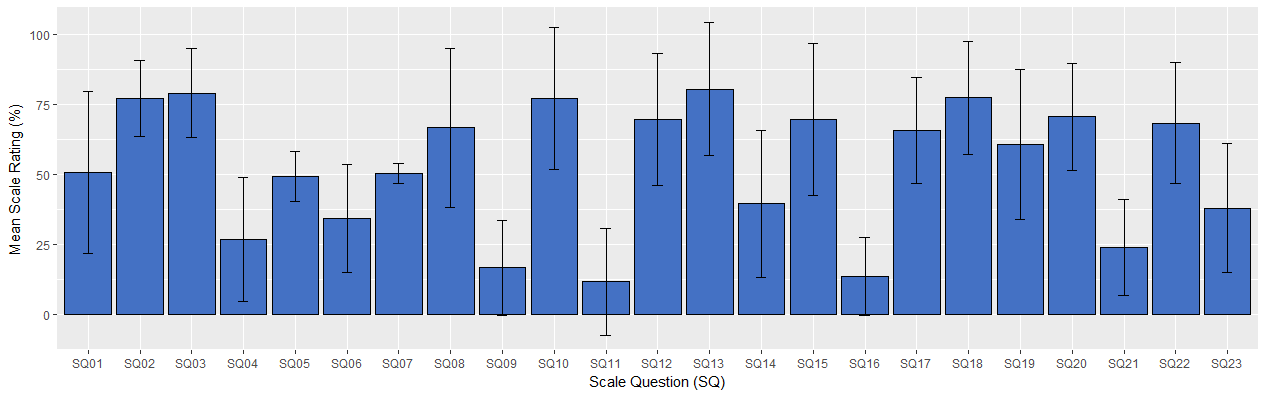
\includegraphics[width = \textwidth]{Figure/DatabehandlingSkalaer/DataPresentation/MeanBarplot} 
\caption{Søjlediagram over den gennemsnitlige besvarelse (\%) til hvert skala spørgsmål (SQ).}
\label{fig:BarPlotGennemsnit}
\end{figure}
\noindent
%
På \autoref{fig:BarPlotGennemsnit} fremgår den gennemsnitlige besvarelse for hver af de 23 skalaer, angivet med \textit{SQ} efterfulgt af nummer.\blankline
%
Der er lavet et kombineret histogram og normalfordelingsplot for hver skala, for at få en forståelse for, hvordan besvarelserne er fordelt. Enkelte af dem vil blive diskuteret i dette afsnit, men de er også alle samlet i \fullref{ElektroniskBilagHistNormal}.

\begin{figure}[H]
\centering
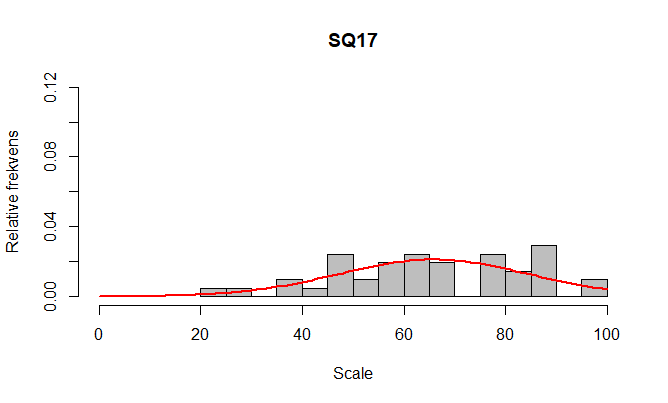
\includegraphics[width = \textwidth]{Figure/DatabehandlingSkalaer/HistogramNormalFordeling/SQ17} 
\caption{Histogrammet viser hyppigheden af besvarelser (y-aksen), inden for de fastsatte intervaller (x-aksen). Den røde kurve viser den underliggende normalfordelingskurve, som er baseret på middelværdien og standardafvigelsen}
\label{fig:histogram17}
\end{figure}
\noindent
%
På \autoref{fig:histogram17} ses et eksempel på et af histogrammerne med tilhørende normalfordelingskurve. Da en stor del af data befinder sig under den røde kurve, tyder det på at besvarelserne for skalaspørgsmål 17 er tilnærmelsesvist normalfordelte. Det undersøges dog ikke med signifikanstest, da formålet med gennemgangen blot er at få et overblik over fordelingerne.\blankline
%
Kurverne i flere af plottene er meget flade, hvilket skyldes at akserne holdes konstante på tværs af plottene, for bedre at kunne sammenligne dem indbyrdes. Det er dog med undtagelse af SQ5 og SQ7, da data er så centreret på disse, at det bliver svært at se fordelingerne på de andre plots hvis akserne defineres ud fra SQ5 og SQ7.\blankline
%
I mange af plottene er der en ret stor varians, hvilket viser at en stor del af skalaen er blevet anvendt. Her skal det tilføjes at besvarelserne er givet ud fra forskellige højder, indfaldsvinkler og afstande og at variansen derfor ikke nødvendigvis er et udtryk for at folk er uenige, men snarere at de har vurderet forskellige stimuli. Et eksempel er givet på \autoref{fig:histogram14}.\blankline
%
\begin{figure}[H]
\centering
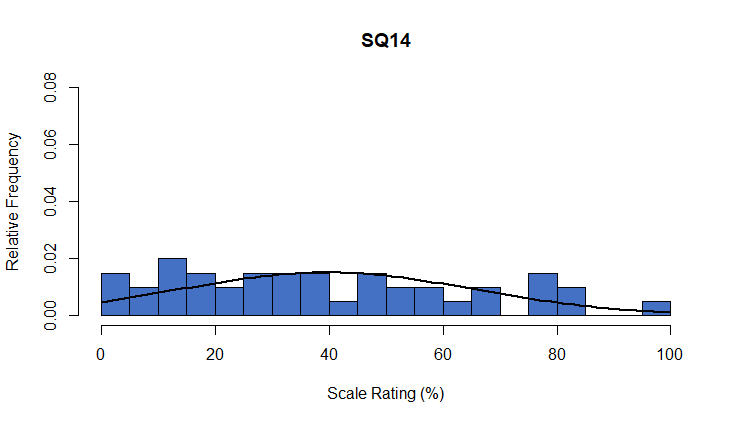
\includegraphics[width = \textwidth]{Figure/DatabehandlingSkalaer/HistogramNormalFordeling/SQ14} 
\caption{Fordelingerne af besvarelserne på skalaspørgsmål 14}
\label{fig:histogram14}
\end{figure}
\noindent
%
I disse historgram- og normalfordelingsplot blev der kigget på, hvordan besvarelserne er fordelt for hvert enkelt spørgsmål, men for at få et samlet overblik, kigges på \autoref{fig:boksplots}, hvor der er lavet boksplots for alle skalaspørgsmålene. \fxnote{Sæt det nye billede for boksplots ind og skriv om det}
%
\begin{figure}[H]
\centering
\includegraphics[width = \textwidth]{Figure/DatabehandlingSkalaer/boksplot0er} 
\caption{Boksplot over fordelinger af besvarelserne for hvert skalaspørgsmål.}
\label{fig:boksplots}
\end{figure}
\noindent
%

Boksplottet deler alle besvarelserne for det pågældende skalaspørgsmål op i fire kvartiler. Medianen adskiller de to midterste kvartiler, og kanterne på kasserne adskiller disse fra de to yderste kvartiler. Outliers er ikke medregnet i kvartilerne for boksplottet, men er stadig plottet for at give en idé om hvordan de fordeler sig i forhold til resten af besvarelserne. \blankline
%
Ud fra boksplottet på \autoref{fig:boksplots} kan det ses at fordelingerne adskiller sig ret meget fra hinanden. Nogle af dem udnytter en stor del af skalaen (1, 4, 8, 12, 14, 19, 22, 23), hvor andre fordeler sig over mindre områder af skalaen (2, 3, 5, 7, 9, 11, 13, 16). Nogle ser tilnærmelsesvis normalfordelte ud (1, 2, 6, 17, 20, 21), hvor andre er skæve enten den ene eller anden vej (8, 9, 10, 11, 13, 18). Der ses også enkelte boksplots hvor datapunkterne ophober sig meget omkring endepunkterne eller midtpunktet (5, 7, 9, 10, 11, 13). \blankline
%
Den lave varians som ses i flere af boksplottene, kan skyldes flere forskellige ting. Det kan enten skyldes at variablen ikke er vigtig for oplevelsen af interaktion og at folk derfor har svaret neutralt. Det kan også skyldes at det ikke er en variabel som er blevet påvirket af de specifikke stimuli som testpersonerne blev udsat for, men at den kan være vigtig i andre situationer med robotten. Effekten forstærkes især ved 5 og 7, som er bipolare skalaer, da midtpunkterne på disse skalaer kan fungere som et anker, som testpersoner ofte vil centrere deres vurderingerne omkring. Labellet ”Fin” som anvendes i spørgsmål 7 blev valgt, da det var testpersonerne fra første tests egne ord. Det kan dog være at beskrivelsen ”Fin” dækker over et for stort spænd af skalaen, og at folk derfor har valgt at sætte stregen lige på midten, selvom robotten måske har været en lille smule for høj eller lav. Dette kan også være med til at centrere datapunkterne omkring midtpunktet og dermed mindske variansen i vurderingerne. \blankline
%
De lukkede endepunkter som blev anvendt på skalaerne, kan være med til at gøre at data ophobes meget omkring disse. Ophobningen af data omkring endepunkterne betyder også at fordelingen bliver skævvredet, da den ofte stopper brat i den ende med endepunktet, men har en lang hale i den anden ende.  \blankline
%
Nogle steder bruges kun øverste halvdel, hvor der andre steder kun bruges nederste halvdel. Det hænger sammen med formuleringerne på endepunkterne, da den positive label sommetider vil være ved 100 (Eks.: ekstremt sød) og i andre tilfælde ved 0 (Eks.: slet ikke anmassende).


\subsection{Varians}
%
For at få et overblik over hvor meget besvarelserne variere og hvor stor forskel, der er mellem variationen ved de forskellige SQ, beregnes variansen for hver SQ beregnes med formlen: \blankline
%
\begin{equation}
	Var = \frac{\sum_{i=1}^{n}(x_i-\overline{x})^{2}}{(n-1)}
\end{equation}
\noindent
%
\fxnote{Indsæt kilde (Field bog)}
Hvor $Var$ er varians, $x_i$ er målingen for nummer $i$, $\overline{x}$ er middelværdien og $n$ er antal målinger. 
En oversigt over variansen for hver SQ kan ses på \autoref{fig:Varians}. 
%
\begin{figure}[H]
\centering
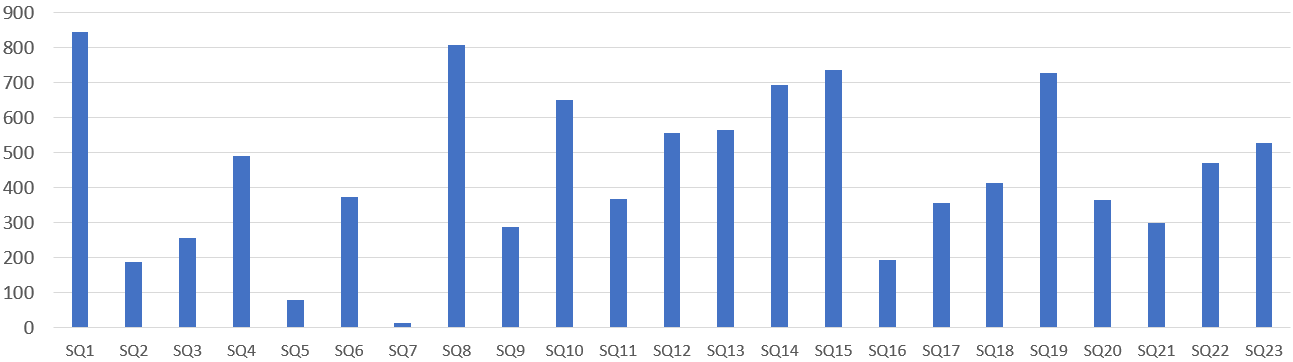
\includegraphics[width = \textwidth]{Figure/DatabehandlingSkalaer/Varians} 
\caption{Søjlediagram over variansen for besvarelserne til hvert Scale Question.}
\label{fig:Varians}
\end{figure}
\noindent
%
Det tydeligt at se ud fra \autoref{fig:Varians} at der er stor forskel mellem variansen ved de forskellige SQ. For eksempel er variansen for SQ5 og SQ7 meget lav i forhold til SQ1 og SQ8. 
%
\subsection{Standardisering af besvarelser}
Når variansen ikke er ens for ens data kan det i nogle tilfælde vælges at udligne variansen. Hvis variansen skulle udlignes vil der skulle laves en standardisering af data. Formålet med at gøre dette er at data med lav varians i rå data får lige betydning i PCA som rå data med stor varians. \blankline
%
Det vælges ikke at standardisere data, da det kan give skævvridninger som ikke er ønsket. Testpersonerne har reelt haft muligheden for at besvarer på hele skalaen, men har valgt at give besvarelser i nærheden af hinanden, hvilket tolkes som at de har været mere enige i dette tilfælde. \blankline
%
Al data er målt med samme måleenhed, da det er målt på samme skala, der går fra 0 til 100 ved aflæsningen. Dette er en del af begrundelsen for ikke at standardisere, da det ofte gøre i tilfælde hvor målingerne ikke er målt med samme måleenhed. \blankline
%
Hvis der er større variation ved nogle skalabesvarelser, vil de vægte mere i en PCA, men det vurderes at være acceptabelt og ønsket. Det er dog vigtigt at være opmærksom på dette, når resultaterne af PCA analyseres. 
